% !TeX root = ../Formelsammlung.tex
\section{Relativsysteme, Inertialsysteme und Relativitätstheorie}
\subsection{Transformation zwischen Bezugssystemen}
\begin{center}
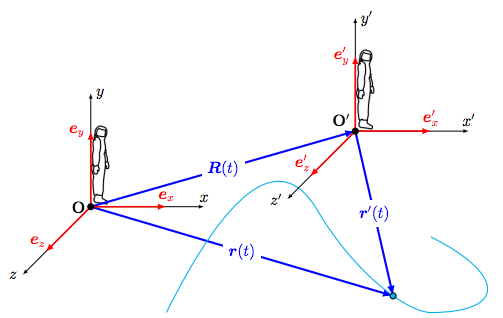
\includegraphics[scale=0.5]{./images/Bezugssysteme.png}
\end{center}
\begin{equation}
\begin{cases}
\vec{r} (t) = \vec{R} (t) + \vec{r^\prime} (t^\prime) \\
t = t^\prime
\end{cases}
\qquad
\begin{cases}
\vec{r^\prime} (t^\prime) = - \vec{R} (t) + \vec{r} (t) \\
t^\prime = t
\end{cases}
\end{equation}
\begin{equation}
\vec{v}(t) = \diff{\vec{R}(t)}{t} + \vec{v^\prime} (t)
\end{equation}
\begin{equation}
\vec{a}(t) = \multidiff{\vec{R}(t)}{t}{2} + \vec{a^\prime} (t)
\end{equation}
\subsection{Inertialsysteme}
Ein Bezugssystem in dem die Newtonschen Gesetze gelten wird Inertialsystem genannt. Das heisst, dass sich verschiedene Inertialsysteme relativ zueinander mit konstanter Geschwindigkeit bewegen.
\subsection{Beschleunigte Systeme, Scheinkräfte}
Wird ein Körper in einem Inertialsystem beschleunigt so gilt $\vec{F} = m \vec{a}$. In einem beschleunigten Bezugssystem gilt jedoch:
\begin{equation}
\vec{F} \neq m \vec{a^\prime} = m \left( \vec{a} - \multidiff{\vec{R}(t)}{t}{2} \right)
\end{equation}
aber:
\begin{equation}
\vec{F^\prime} = m \vec{a^\prime} = m \left( \vec{a} - \multidiff{\vec{R}(t)}{t}{2} \right) \quad\Rightarrow\quad \vec{F^\prime} = \vec{F} + \underbrace{\multidiff{\vec{R}(t)}{t}{2}}_{\text{Scheinkraft}}
\end{equation}
\subsubsection{Rotierendes Bezugssytem}
Annahme: $\omega$ konstant. 
\paragraph{Die Zentrifugalkraft}
\begin{equation}
\vec{F}_{ZP} = m \left(r^\prime \omega ^2 \right) \e{r}
\end{equation}
\paragraph{Die Corioliskraft}
\begin{equation}
\vec{F}_{C} = m \left(2 v^\prime \omega \right) \e{\varphi}
\end{equation}
\subsection{Galileitransformation}
Betrachtet werden 2 Bezugssysteme die sich relativ zueinander mit konstanter Geschwindigkeit $\vec{V}$ bewegen.
\begin{align}
\vec{r^\prime}(t) &= \vec{r} (t) - \vec{V} t \\
\vec{v^\prime} &= \vec{v} - \vec{V} \\
\vec{a^\prime}(t) &= \vec{a}(t)
\end{align}
\subsubsection{Raumzeit}
\begin{equation}
x^\mu \equiv 
\begin{pmatrix}
ct & x & y & z
\end{pmatrix}
\end{equation}
Die Galileitransformation kann nun so geschrieben werden:
\begin{equation}
\underbrace{
\begin{pmatrix}
ct^\prime \\
x^\prime \\
y^\prime \\
z^\prime
\end{pmatrix}
}_{x^{\prime \mu}}
= 
\underbrace{
\begin{pmatrix}
1 		& 0 & 0 & 0 \\
-\beta 	& 1 & 0 & 0 \\
0		& 0 & 1 & 0 \\
0		& 0 & 0 & 1
\end{pmatrix}
}_{M_G (\beta)}
\underbrace{
\begin{pmatrix}
ct \\
x \\
y \\
z
\end{pmatrix}
}_{x^\mu}
\end{equation}
Die Inverse lautet:
\begin{equation}
\underbrace{
\begin{pmatrix}
ct \\
x \\
y \\
z
\end{pmatrix}
}_{x^\mu}
= 
\underbrace{
\begin{pmatrix}
1 		& 0 & 0 & 0 \\
+\beta 	& 1 & 0 & 0 \\
0		& 0 & 1 & 0 \\
0		& 0 & 0 & 1
\end{pmatrix}
}_{M_G^{-1} (\beta)}
\underbrace{
\begin{pmatrix}
ct^\prime \\
x^\prime \\
y^\prime \\
z^\prime
\end{pmatrix}
}_{x^{\prime \mu}}
\end{equation}
\subsection{Lorentztransformation}
\begin{equation}
\begin{pmatrix}
ct^\prime \\
x^\prime \\
y^\prime \\
z^\prime
\end{pmatrix}
= 
\begin{pmatrix}
\gamma			& -\beta \gamma	& 0 & 0 \\
-\beta \gamma	& \gamma			& 0 & 0 \\
0		& 			0 			& 1 & 0 \\
0		& 			0 			& 0 & 1
\end{pmatrix}
\begin{pmatrix}
ct \\
x \\
y \\
z
\end{pmatrix}
\end{equation}
Für die Inverse gilt wiederum:
\begin{equation}
\begin{pmatrix}
ct \\
x \\
y \\
z
\end{pmatrix}
= 
\begin{pmatrix}
\gamma			& +\beta \gamma	& 0 & 0 \\
+\beta \gamma	& \gamma			& 0 & 0 \\
0		& 			0 			& 1 & 0 \\
0		& 			0 			& 0 & 1
\end{pmatrix}
\begin{pmatrix}
ct^\prime \\
x^\prime \\
y^\prime \\
z^\prime
\end{pmatrix}
\end{equation}
\subsection{Die Raumzeit}
Da bei relativistischem Ansatz:
\begin{equation}
\Delta t \neq \Delta t^\prime \quad\Rightarrow\quad \Delta x \neq \Delta x^\prime \quad\Rightarrow\quad \Delta r \neq \Delta r^\prime
\end{equation}
(Von verschiedenen Beobachteren gemessene Zeitintervalle zwischen zwei Ereignissen sind nicht immer gleich). Das Raumzeit-Intervall $\Delta s$ ist jedoch für alle Beobachter identisch. 
\begin{equation}
\begin{split}
\Delta s ^2 	& \equiv (c \Delta t)^2 - \Delta r ^2 \\
			& = (c \Delta t)^2 - \Delta x ^2 - \Delta y ^2 - \Delta z ^2
\end{split}
\end{equation}
\subsubsection{Zeitdilatation}
Ist $\Delta \tau $ die in einem unbewegten System gemessene Zeitdifferenz zwischen zwei Ereignissen so gilt in einem bewegten System für die Zeitdifferenz $\Delta t$:
\begin{equation}
\Delta t = \gamma \cdot \Delta \tau
\end{equation}
\subsubsection{Längenkontraktion}
Da für bewegte Systeme bezüglich unbewegten die Zeit langsamer vergeht, müssen in einem bewegten System auch die Distanzen bezüglich dem unbewegten System kürzer werden. \\
Beispiel: Eine Raktete fliegt mit einer Gewschwindigkeit für die $\gamma = 10$ gilt zu einem für uns 100 Lichtjahre entferneten Planeten. Da die Rakete sich bewegt vergeht in ihr die Zeit langsamer bezüglich der Erde. Sie kann den Planeten darum in 10 Lichtjahren erreichen (Zeitdilatation). Die Strecke die die Rakete dabei zurücklegt ($\gamma = 10 \Rightarrow v \approx c$) beträgt 10 Lichtjahre. Die Länge ist kontrahiert! \\
Ist die ursprüngliche Länge $\Delta \lambda$ so gilt für die Länge $\Delta x$ in einem bewegten System:
\begin{equation}
\Delta x = \dfrac{\Delta \lambda}{\gamma}
\end{equation}
\subsection{Geschwindigkeitstransformation}
Ein Körper K bewegt sich im Bezugssystem $\mathbf{O^\prime}$ mit einer Geschwindigkeit $\vec{u^\prime}$. $\mathbf{O^\prime}$ bewegt sich bezüglich $\mathbf{O}$ mit der Geschwindigkeit $V$ in x-Richtung. K bewegt sich bezüglich $\mathbf{O}$ mit einer Geschwindigkeit $\vec{u}$:
\begin{align}
u_x &= \cfrac{u_x^\prime + V}{1 + \frac{\beta}{c} u_x^\prime} \\
u_y &= \cfrac{u_y^\prime}{\gamma \left( 1 + \frac{\beta}{c}u_x^\prime \right)} \\
u_z &= \cfrac{u_z^\prime}{\gamma \left( 1 + \frac{\beta}{c}u_x^\prime \right)}
\end{align}